\documentclass[border=0.5cm,letterpaper]{standalone}
\usepackage{tikz}
\usetikzlibrary{positioning}
\begin{document}

\tikzset{%
  every neuron/.style={
    circle,
    draw,
    minimum size=1cm
  },
  neuron missing/.style={
    draw=none, 
    scale=4,
    text height=0.333cm,
    execute at begin node=\color{black}$\vdots$
  },
}

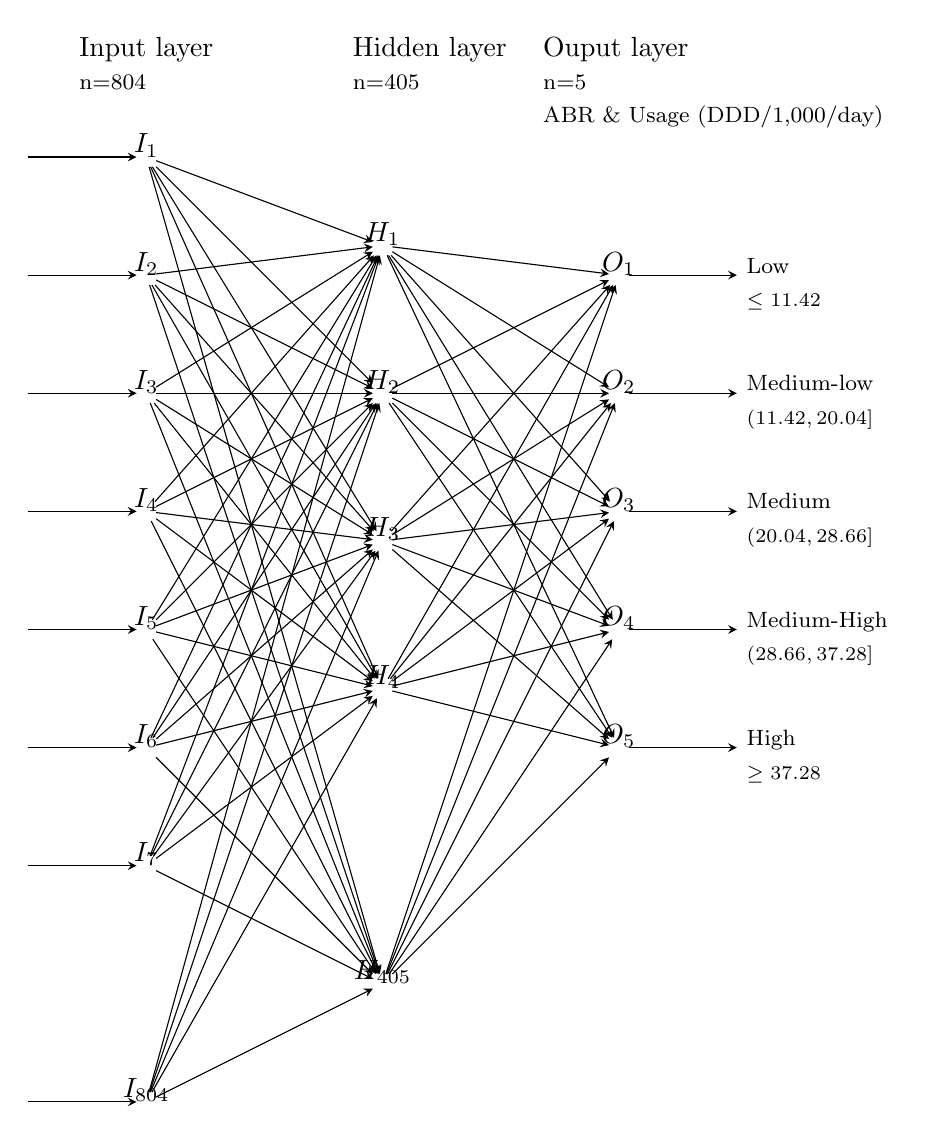
\begin{tikzpicture}[x=1.5cm, y=1.5cm, >=stealth]

\foreach \m/\l [count=\y] in {1,2,3,4,5,6,7,missing,8}
  \node [every neuron/.try, neuron \m/.try] (input-\m) at (0,2.5-\y) {};

\foreach \m [count=\y] in {1,2,3,4,missing,5}
  \node [every neuron/.try, neuron \m/.try ] (hidden-\m) at (2,2-\y*1.25) {};

\foreach \m [count=\y] in {1,2,3,4,5}
  \node [every neuron/.try, neuron \m/.try ] (output-\m) at (4,1.5-\y) {};

\foreach \l [count=\i] in {1,2,3,4,5,6,7,804}
  \draw [<-] (input-\i) -- ++(-1,0)
    node [above] at (input-\i.south) {$I_{\l}$};

\foreach \l [count=\i] in {1,2,3,4,405}
  \node [above] at (hidden-\i.south) {$H_{\l}$};

\foreach \l [count=\i] in {1,2,3,4,5}
  \node [above] at (output-\i.south) {$O_{\l}$};

\foreach \l [count=\i] in {{1,2,3,4,5,6,7,8}}
  node [align=left, right] {\\\l};

\foreach \l [count=\i] in {{\footnotesize{Low}\\\scriptsize{$\leq 11.42$}}, {\footnotesize{Medium-low}\\\scriptsize{$(11.42, 20.04]$}}, {\footnotesize{Medium}\\\scriptsize{$(20.04, 28.66]$}}, {\footnotesize{Medium-High}\\\scriptsize{$(28.66, 37.28]$}}, {\footnotesize{High}\\\scriptsize{$\ge 37.28$}}}
  \draw [->] (output-\i) -- ++(1,0)
  node [align=left, right] {\\\l};

\foreach \i in {1,...,8}
  \foreach \j in {1,...,5}
    \draw [->] (input-\i) -- (hidden-\j);

\foreach \i in {1,...,5}
  \foreach \j in {1,...,5}
    \draw [->] (hidden-\i) -- (output-\j);

\foreach \l [count=\x from 0] in {Input layer\\\footnotesize{n=804}, Hidden layer\\\footnotesize{n=405}, Ouput layer\\\footnotesize{n=5}\\\footnotesize{ABR \& Usage (DDD/1,000/day)}}
  \node [align=left, below] at (\x*2.4,2.6) {\l};

\end{tikzpicture}

\end{document}